
\section{Introduccion}
El presente informe describe el desarrollo e implementación de un sistema de manejo de caché denominado Least Recently Used (LRU), 
cuyo objetivo es optimizar el uso de memoria reemplazando los datos menos utilizados recientemente.\\
Este proyecto fue desarrollado en lenguaje C como parte del curso Estructuras de Datos, utilizando estructuras como () para gestionar el almacenamiento y 
la prioridad de los datos.\\
A través de esta implementación se busca comprender el funcionamiento de un algoritmo de reemplazo de caché y aplicar conceptos 
fundamentales como el manejo dinámico de memoria, el uso de punteros y la eficiencia algorítmica.\\
Este proyecto se desarrolló de manera colaborativa mediante el uso de Git, creando un repositorio en GitHub. Además, 
se aprovechó la extensión Live Share de Visual Studio Code para facilitar el trabajo en tiempo real entre los integrantes del equipo.
\newpage
\section{Objetivos}
\begin{itemize}
    \item Comprender el funcionamiento del algoritmo LRU (Least Recently Used).
    \item Implementar estructuras de datos abstractas como [] para la gestión del caché.
    \item Desarrollar habilidades en programación en lenguaje C, especialmente en el manejo de memoria y punteros.
    \item Simular el comportamiento de un sistema de caché limitado en tamaño, que reordene y elimine datos de acuerdo con su uso reciente.
\end{itemize}
\newpage
\section{Estructuras de Datos Utilizadas}
Para la implementación del sistema de caché LRU, se utilizaron las siguientes estructuras de datos:
\begin{itemize}
    \item Lista enlazada (Linked List)
    \item Puntero
    \item Funciones de manipulación de nodos
\end{itemize}
    \subsection{Puntero}
    Un puntero en informática (y en lenguajes como C o C++) es una variable que almacena la dirección de memoria de otra variable, en lugar de almacenar directamente un valor.
    Los punteros se utilizan para:
    \begin{itemize}
        \item Acceder y modificar valores indirectamente:
            \begin{lstlisting}[style=CodeStyle, language=C, caption={Acceder y modificar valores indirectamente}, label={lst:codigo}]
            *ptr = 20; // Cambia el valor de x a 20
            \end{lstlisting}
        \item Listas enlazadas, árboles y grafos
        \item Paso de parámetros por referencia: Permite que una función modifique la variable original
            \begin{lstlisting}[style=CodeStyle, language=C, caption={Paso de parámetros por referencia}, label={lst:codigo}]
                void incrementar(int *p) { *p = *p + 1; }
            \end{lstlisting}
        \item Memoria dinamica
        \item Eficiencia
    \end{itemize}
    A continuación, se muestra una imagen que ilustra el concepto de puntero:
    \begin{figure}[H]
        \centering % Para que aparezca centrada
        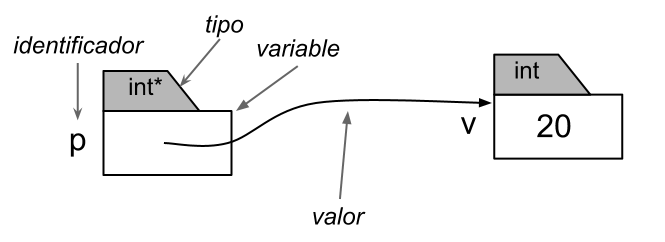
\includegraphics[width=0.5\textwidth]{./src/images/puntero.png} 
        \caption{Puntero} 
        \label{fig: puntero} 
    \end{figure}

    \subsection{Lista Enlazada}
    Una \textbf{lista enlazada} es una estructura de datos dinámica que consiste en una serie de elementos llamados nodos, donde cada nodo contiene un dato y una referencia 
    al siguiente nodo en la secuencia. A diferencia de un array, las listas enlazadas permiten un crecimiento dinámico sin un tamaño fijo y facilitan la inserción 
    y eliminación de elementos, ya que solo requieren actualizar referencias.\\

    Sin embargo, las listas enlazadas presentan tanto ventajas como desventajas frente a los arreglos:
    \begin{itemize}
        \item \textbf{Ventajas:} Inserciones y eliminaciones en cualquier posición sin necesidad de mover todos los elementos. Crecimiento dinámico sin tamaño predefinido.
        \item \textbf{Desventajas:} La búsqueda de un dato específico requiere recorrer la lista nodo por nodo ($O(N)$), mientras que en un arreglo, si se conoce el índice, se puede acceder directamente en $O(1)$.
    \end{itemize}
    
    Para comprender mejor una lista enlazada es importante saber que es un nodo.
        \subsubsection{Nodo}
        En informática, un nodo es un elemento individual de una estructura de datos que almacena información y, en muchos casos, tiene referencias o enlaces a otros nodos. 
        Los nodos son la base de muchas estructuras de datos dinámicas, como listas enlazadas, árboles y grafos.\\
        Un nodo tiene dos componentes principales:
        \begin{itemize}
            \item  \textbf{Dato}: La información que el nodo almacena, que puede ser de cualquier tipo de dato, como un número, una cadena de texto o un objeto más complejo.
            \item  \textbf{Referencia}:Un puntero o referencia al siguiente nodo en la lista
        \end{itemize}
        En la siguiente imagen se puede apreciar de manera grafica que es un nodo
        \begin{figure}[H]
            \centering % Para que aparezca centrada
            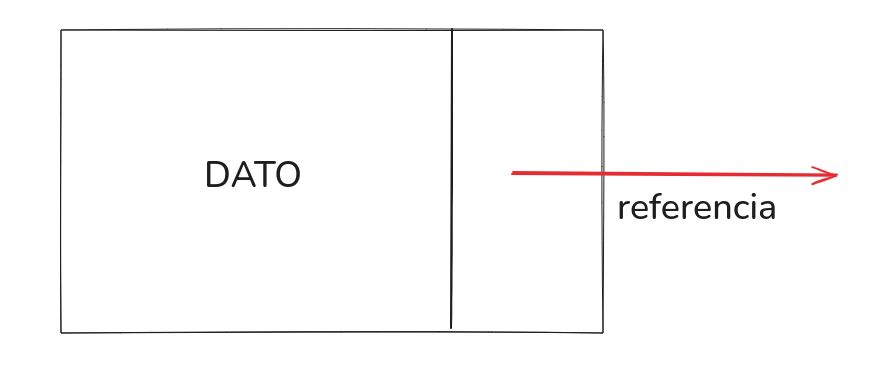
\includegraphics[width=0.5\textwidth]{./src/images/Nodo.png} 
            \caption{Nodo} 
            \label{fig: nodo} 
        \end{figure}
    Las listas enlazadas tienen un nodo inicial llamado \textbf{head} el cual apunta al primer elemento de la lista. Si se llega a un nodo que no apunta a ningún otro, 
    se dice que dicho nodo apunta a \textbf{null} o final de la lista.\\
    En la siguiente imagen se puede apreciar de manera grafica que es una lista enlazada
    \begin{figure}[H]
        \centering % Para que aparezca centrada
        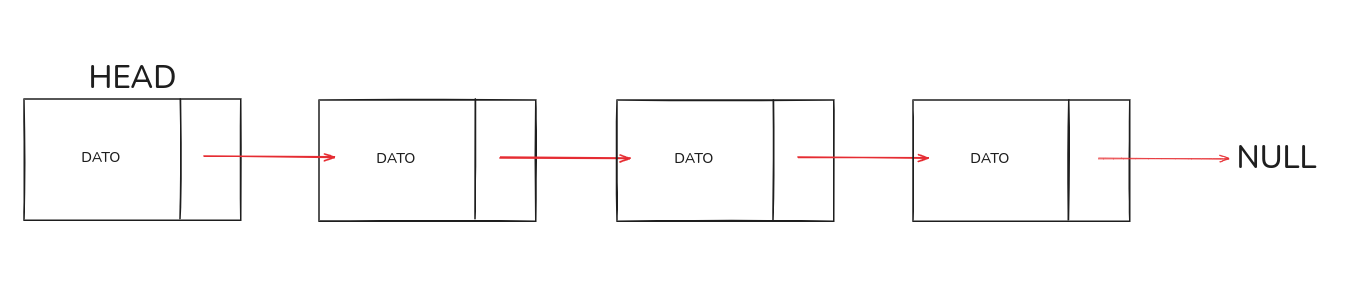
\includegraphics[width=0.9\textwidth]{./src/images/ListaEnlazada.png} 
        \caption{Lista enlazada} 
        \label{fig: lista} 
    \end{figure}
    Se utilizó una lista enlazada para mantener el orden de los elementos en la caché, permitiendo una fácil inserción, eliminación y reordenamiento de los nodos 
    según su uso reciente, de esta manera se garantiza que los datos más utilizados recientemente se encuentren en la parte superior de la lista, mientras que los 
    datos menos utilizados se encuentren en la parte inferior.
    \subsubsection{Implementacion mediante Lista Enlazada}
    La lista enlazada (o lista ligada simple), definida por las estructuras en \texttt{nodes.h} y gestionada por \texttt{LRUcache}, 
    es la \textbf{estructura de datos central} que implementa la cache LRU. Su funcion va mas alla del simple almacenamiento: es el mecanismo que mantiene el 
    orden de recencia de uso (uso reciente).
    \paragraph{Mantenimiento del Orden de Recencia (MRU $\rightarrow$ LRU)}
    La lista se manipula estrictamente para que sus extremos reflejen la recencia de uso:
    \begin{itemize}
        \item \textbf{Inicio de la Lista}: Representa el \textbf{Most Recently Used} (MRU), accesible en $O(1)$ mediante el puntero \texttt{cache->primero}.
        \item \textbf{Final de la Lista}: Representa el \textbf{Least Recently Used} (LRU), accesible en $O(1)$ mediante el puntero \texttt{cache->ultimo}.
    \end{itemize}

    \paragraph{Uso en la Logica de la Cache}
    La lista enlazada es esencial para todas las operaciones clave de la cache:
    \begin{itemize}
        \item \textbf{Insercion/Reubicacion}: Las operaciones de agregar y usar un dato siempre implican mover el nodo al inicio de la lista para reflejar el nuevo estado MRU.
        \item \textbf{Desalojo}: La eliminacion del LRU se realiza directamente desde el final de la lista, ya que es el candidato menos recientemente usado.
    \end{itemize}

    \subsection{Manipulacion de Nodos}
    La manipulacion de los nodos fue fundamental para implementar la politica LRU, asegurando que la lista ligada mantuviera el orden de recencia de uso. Los nodos son gestionados directamente mediante punteros para mantener al inicio el MRU y al final el LRU.

        \subsubsection*{Reubicacion de Uso (Reubicacion MRU)}
        Cuando se accede a un nodo existente (\texttt{usar\_dato}), este debe ser movido a la posicion MRU. El proceso implica:
        \begin{enumerate}
            \item Localizar el nodo (\texttt{actual}) y su predecesor (\texttt{prev}). Esta busqueda es $O(N)$.
            \item \textbf{Desvincular}: El puntero \texttt{prev->Next} se salta \texttt{actual}.
            \item \textbf{Re-insertar al inicio}: El nodo \texttt{actual} se convierte en el nuevo \texttt{cache->main->Next}.
            \item \textbf{Actualizacion de LRU}: Si el nodo movido era el \texttt{cache->ultimo}, el puntero se actualiza a \texttt{prev}.
        \end{enumerate}

        \subsubsection*{Eliminacion del Menos Usado (LRU)}
        El desalojo se activa cuando la capacidad se excede. Se elimina el nodo al final de la lista.
        \begin{itemize}
            \item Se recorre la lista hasta encontrar el penultimo nodo (\texttt{prev}) que precede al LRU (\texttt{actual}).
            \item El LRU es desvinculado al hacer que \texttt{prev->Next} apunte a \texttt{NULL}.
            \item El puntero \texttt{cache->ultimo} se establece a \texttt{prev}.
            \item Se libera la memoria del nodo eliminado (\texttt{free(actual)}).
        \end{itemize}

        \subsubsection*{Mecanismo de Carga}
        Para reconstruir la cache desde el disco sin alterar el orden guardado, se utiliza la funcion auxiliar \texttt{insertar\_al\_final}. 
        Esta funcion anade nodos directamente utilizando \texttt{cache->ultimo} en $O(1)$, evitando la logica de reubicacion MRU de \texttt{agregar\_dato}.

    \subsection{Estructura de la Cache LRU (\texttt{LRUcache})}
    La gestion de la lista enlazada y el control de la capacidad se centralizan en la estructura \texttt{LRUcache}, definida en \texttt{lru.h}.

    \begin{lstlisting}[caption=Estructura de Control LRUcache, language=C, label=lst:LRUcache]
    typedef struct {
        int max_cache;
        List main;
        Position primero;
        Position ultimo;
    } LRUcache;
    \end{lstlisting}

    \begin{itemize}
        \item \textbf{\texttt{max\_cache}}: Almacena la capacidad maxima permitida para la cache.
        \item \textbf{\texttt{main} (List)}: Puntero al nodo cabecera de la lista enlazada, sirviendo como punto de acceso para todas las operaciones.
        \item \textbf{\texttt{primero} (Position)}: Puntero auxiliar que apunta directamente al nodo \textbf{Mas Recientemente Usado (MRU)}. Facilita la insercion en $O(1)$.
        \item \textbf{\texttt{ultimo} (Position)}: Puntero auxiliar que apunta directamente al nodo \textbf{Menos Recientemente Usado (LRU)}. Facilita la eliminacion por desalojo en $O(1)$ una vez localizado su predecesor.
    \end{itemize}
\newpage
\section{Implementacion de comandos}
    \subsection{Lru create N}
    EEste comando se encarga de crear la memoria cache y designar un máximo de elementos dentro del mísmo. 
    \textbf{¿Cómo lo hace?} En primer lugar, se implemento el uso de argumentos, y estos se ingresan como argumento 
    para la función que está condicionada con un if, ya que, si en la ejecución de la función, existe un error, 
    entonces la función completa devolverá 1, y por consecuencia, main.c también lo hará. Luego, se crearán:
    \begin{itemize}
        \item lru\_cache (carpeta)
        \item metadata.txt
        \item data.txt
    \end{itemize}
    En metadata.txt se guardarán los datos del cache, mientras que en data.txt, se guardará el orden de la lista enlazada.
    \subsection{Lru add\_data} % Esto sería un subtítulo
    Este comando añade elementos al cache actual (Se añaden elementos a la lista). En cada llamada de la función, primero se cargarán los datos del cache. 
    Luego, se asegura de que, si el dato que se quiere ingresar ya existe, entonces encuentra ese nodo, y lo marca como usado (\textbf{MRU: Most Recently Used}). 
    De no ser así, contará la cantidad de datos actuales, la comparará con la cantidad máxima, y de ser excedida esa capacidad, entonces eliminará el dato menos usado 
    con la función ''eliminar\_menos\_usado''.
    \subsection{Lru get data \textless data\textgreater}
    Esta función cumple el rol de 'Usar' un dato especificado, así se cambiará su lugar en la lista enlazada, marcado como \textbf{MRU} (Most Recently Used). 
    Para ello, primero \textbf{buscará} el dato ingresado mediante un bucle \texttt{while} (Función \texttt{FindNode}), que tiene una complejidad de $O(N)$. 
    Si el dato ya es MRU (\texttt{cache->primero}), entonces devolverá un mensaje sin realizar movimientos. Del contrario y una vez encontrado,
    se \textbf{invierte su recencia} a través de la función \texttt{usar\_dato}.
    \begin{enumerate}
        \item \textbf{Desvinculación}: Se desvincula el nodo encontrado de su posición actual mediante la actualización de los punteros \texttt{Next} de su nodo predecesor.
        \item \textbf{Reubicación}: El nodo es re-insertado inmediatamente al inicio de la lista (después de la cabecera) para establecerlo como el nuevo \textbf{MRU}. El puntero \texttt{cache->primero} es actualizado.
        \item \textbf{Persistencia}: Finalmente, el nuevo orden de la lista enlazada es \textbf{guardado} en el archivo \texttt{data.txt}, garantizando que el estado de recencia actualizado se conserve en el disco.
    \end{enumerate}
    Este proceso es fundamental para la política LRU, ya que garantiza que los datos consultados mantengan su prioridad y no sean desalojados prematuramente.
\section{Persistencia y Manejo de Archivos}
    La \textbf{persistencia} es la cualidad de los datos de \textbf{sobrevivir más allá del ciclo de vida del programa} que los creó o manipula. En este proyecto, 
    garantiza que el estado y el orden de recencia (\textbf{MRU $\rightarrow$ LRU}) de la caché se mantengan entre diferentes ejecuciones del programa.
    \subsection{Estructura de Persistencia}
    La cache utiliza el sistema de archivos del sistema operativo para lograr la persistencia, basándose en la siguiente estructura:
    \begin{itemize}
        \item \textbf{Directorio \texttt{lru\_cache}}: Contiene todos los archivos de la cache. La creacion se maneja por la funcion \texttt{CreateDir}.
        \item \textbf{\texttt{metadata.txt}}: Archivo que almacena informacion estatica, principalmente la capacidad maxima (\texttt{max\_cache}).
        \item \textbf{\texttt{data.txt}}: Archivo donde se guardan los datos de la lista enlazada, un elemento por linea, manteniendo el orden de recencia (MRU $\rightarrow$ LRU).
    \end{itemize}

    \subsection{Mecanismos de Persistencia (Carga y Guardado)}
    La gestion del estado persistente se logra mediante las siguientes operaciones:
    \begin{itemize}
        \item \textbf{Carga (\texttt{LoadCache})}: Se ejecuta al inicio de cada comando de manipulacion. Lee \texttt{metadata.txt} y \texttt{data.txt}. Utiliza la funcion auxiliar \texttt{insertar\_al\_final} para \textbf{reconstruir la lista en memoria (RAM)} en el orden exacto en que fue guardada, evitando que la logica de reubicacion LRU altere el orden de carga.
        \item \textbf{Guardado (Escritura)}: Despues de cada modificacion (\texttt{add\_data} o \texttt{get data}), el estado actual y orden de la lista enlazada se sobreescribe completamente en \texttt{data.txt} para reflejar la recencia mas reciente de la cache.
    \end{itemize}
\newpage
\section{Conclusion}
La implementacion demostro ser exitosa en simular la politica LRU, utilizando la lista enlazada para mantener la jerarquia de uso. 
La gestion mediante los punteros auxiliares \texttt{primero} y \texttt{ultimo} permitio lograr una complejidad de tiempo eficiente, de $O(1)$ para las operaciones de insercion MRU y eliminacion LRU. 
Sin embargo, la busqueda de datos dentro de la lista sigue siendo de $O(N)$, lo cual podria mejorarse en futuras iteraciones.
Para optimizar el rendimiento del sistema, se podrian realizar los siguientes cambios a futuro:
\begin{itemize}
    \item \textbf{Optimizar Busqueda}: Migrar la implementacion a una \textbf{Lista Doblemente Enlazada} y combinarla con un \textbf{HashMap} (tabla hash). Esto reduciria la complejidad de la busqueda de elementos de $O(N)$ a $O(1)$.
    \item \textbf{Gestion de Errores}: Mejorar el manejo de errores de persistencia y archivos.
\end{itemize}
